% =============================================================================
% 3.3 缺失检索参数的上下文推理与动态补全
% 草稿版本：v0.2 (2026-05-07)
%   v0.1：完成正文初稿。
%   v0.2：按导师意见 8 在 3.3.3 末段嵌入 fig:completion-three-tier
%        三档补全策略流程图，可视化"默认值 → 上下文推断 → 常识"
%        优先级链与失败时触发 follow_up_question 的兜底分支。
% 字数：约 1700 字
% 风格规则：v0.2 风格（无 \textbf / \textit / 引例括号 / 双引号 / 破折号）
% 引用：\cite{ref10, ref15, ref29}
% 图表：
%   - 图 \reffig{fig:completion-three-tier}         三档补全策略流程图
%   - 表 \reftab{tab:completion-required-params}    各意图类型的关键参数清单
%   - 表 \reftab{tab:completion-sources}            四类补全来源
% 依赖宏包：booktabs / tabularx / graphicx（主稿已加载）
% =============================================================================

\subsection{缺失检索参数的上下文推理与动态补全}
\label{sec:param-completion}

前节的 \texttt{recognizer} 解决了把自然语言查询解析为结构化意图的
问题，但实际查询中用户经常省略关键参数。
例如查明天天气怎么样省略了地点、查武汉怎么样省略了时间、查现在适合
洗车吗省略了城市。如果系统直接把这类不完整意图送入 ReAct 循环，会
触发两类失败：一类是模型自行编造缺失参数，例如把缺地点的查询补成
当前位置等虚构城市；另一类是模型按某个默认值兜底但不告诉用户，导致
用户得到与预期不符的回答。本文据此设计了独立的参数补全模块
\texttt{completer}，位于 \texttt{src/\bk{}intent/\bk{}completer.\bk{}py}，承担缺失
参数判定、自动补全、与友好追问三类职责。

\subsubsection*{3.3.1 \quad 分层架构的设计动机}

参数补全在工程上完全可以与意图识别合并到同一个大语言模型调用中
完成，但本文选择把两者切分为独立的两阶段管线，理由源自单点错误
的容错性考虑 \cite{ref10}。意图识别与参数补全在错误模式上具有
不同的特征：意图识别错误通常是分类边界模糊，例如把
\texttt{daily\_\bk{}forecast} 误判为 \texttt{hourly\_\bk{}forecast}；参数
补全错误则通常是字段填充幻觉，例如把没有提及地点的查询补出虚构
城市。两类错误若混合在同一次大语言模型调用中，模型在生成
\texttt{intent} 字段时的注意力分配会与生成 \texttt{locations}
字段时相互干扰。

分层架构允许后置阶段在前置阶段产生抖动时进行业务层兜底。
\ref{sec:intent-eval} 节的 \texttt{index\_\bk{}004\_\bk{}no\_\bk{}loc} 用例提供了
这一容错机制的具体实证。该用例的查询是今天去爬山合适吗，
\texttt{recognizer} 输出 \texttt{intent=\bk{}life\_\bk{}index} 正确判定意图，
但在 \texttt{locations} 字段填入了虚构的当前位置作为礼貌性补白。
\texttt{completer} 阶段识别出当前位置不是合法城市名，触发
\texttt{is\_\bk{}complete=\bk{}False} 与友好追问，最终系统反问用户希望查询
哪个城市。如果不分层，单次大语言模型调用产生地点幻觉后会直接
进入 ReAct 循环并去查虚构城市的生活指数，业务层无从纠正。
这一案例印证了分层架构本身即是容错机制，与 ChatDev \cite{ref29}
中按软件工程瀑布模型把开发任务分阶段交由不同角色协作以减少幻觉
的总体思路在精神上接近。

\subsubsection*{3.3.2 \quad 关键参数清单与判定逻辑}

\texttt{completer} 模块通过显式列出每类意图的关键参数清单来实现
缺失判定，详见 \reftab{tab:completion-required-params}。各意图
类型对参数完整性的要求差异显著：\texttt{current\_\bk{}weather} 仅要求
有地点不要求有时间，因为实时天气默认查当前；
\texttt{travel\_\bk{}advice} 要求至少 2 个地点加完整时间，因为出行场景
本质上是多地点多时段的复合查询。

\begin{table}[!ht]
    \centering
    \caption{各意图类型的关键参数清单}
    \label{tab:completion-required-params}
    \song\fontsize{9pt}{12pt}\selectfont
    \renewcommand{\arraystretch}{0.95}
    \begin{tabular}{ll}
        \toprule
        意图类型 & 关键参数 \\
        \midrule
        \texttt{current\_\bk{}weather} & \texttt{locations} \\
        \texttt{hourly\_\bk{}forecast} & \texttt{locations} + \texttt{time.\bk{}date} \\
        \texttt{daily\_\bk{}forecast} & \texttt{locations} + \texttt{time.\bk{}date} \\
        \texttt{weather\_\bk{}warning} & \texttt{locations} \\
        \texttt{life\_\bk{}index} & \texttt{locations} + \texttt{time.\bk{}date} \\
        \texttt{historical\_\bk{}hourly} & \texttt{locations} + \texttt{time.\bk{}date} 起止日期 \\
        \texttt{historical\_\bk{}daily} & \texttt{locations} + \texttt{time.\bk{}date} 起止日期 \\
        \texttt{travel\_\bk{}advice} & 至少 2 个 \texttt{locations} + \texttt{time} \\
        \bottomrule
    \end{tabular}
\end{table}

\texttt{completer} 把关键参数清单写入 \texttt{COMPLETER\_\bk{}PROMPT}
的结构化系统提示中，以列表形式让大语言模型在每次判定时显式对照。
这一显式枚举的设计避免了模型自行猜测哪些字段是关键的不确定性。
当某个关键参数缺失且无法自动补全时，模型输出
\texttt{is\_\bk{}complete=\bk{}False} 并填写 \texttt{follow\_\bk{}up\_\bk{}question}
字段，例如您想查询哪个城市的生活指数。

\subsubsection*{3.3.3 \quad 三档补全策略与四类补全来源}

对于可推断的缺失参数，\texttt{completer} 使用三档优先级补全策略。
第一档是默认值规则。当用户未指明时间但意图允许时，默认补
\texttt{time.\bk{}date} 等于今天。这一档处理日常查询省略时间的常见
情形。第二档是上下文推断。模块在调用时可选传入
\texttt{conversation\_\bk{}context} 参数，承载历史对话摘要。基于历史
对话推断的典型场景包括用户上一轮问过北京，本轮问那明天呢应补
\texttt{location=\bk{}北京}。第三档是常识推断。例如用户说早上而未指明
具体时刻，模块按行业惯例补 \texttt{start\_\bk{}time=\bk{}06:00}, 
\texttt{end\_\bk{}time=\bk{}09:00}。三档之间的优先级关系是：用户输入优于
上下文推断、上下文推断优于默认值、默认值优于常识推断，避免补全
之间相互覆盖。

每条补全操作都会被写入 \texttt{CompletionResult.\bk{}notes} 字段。
单条记录由 \texttt{field}、\texttt{value}、\texttt{source}、
\texttt{reason} 四个子字段组成。其中 \texttt{source} 取四个枚举值
之一，详见 \reftab{tab:completion-sources}。

\begin{table}[!ht]
    \centering
    \caption{补全记录的四类来源（\texttt{CompletionNote.\bk{}source}）}
    \label{tab:completion-sources}
    \song\fontsize{9pt}{12pt}\selectfont
    \renewcommand{\arraystretch}{0.95}
    \begin{tabular}{ll}
        \toprule
        来源 & 含义 \\
        \midrule
        \texttt{user\_\bk{}input} & 用户在原始查询中明确给出 \\
        \texttt{context\_\bk{}inference} & 从历史对话或前置上下文推断 \\
        \texttt{default} & 使用合理默认值，例如时间默认今天 \\
        \texttt{common\_\bk{}sense} & 基于行业惯例或日常常识推断 \\
        \bottomrule
    \end{tabular}
\end{table}

四类来源在用户体验上的差异是关键工程考虑。\texttt{user\_\bk{}input} 不
需要向用户解释；\texttt{default} 与 \texttt{common\_\bk{}sense} 需要在
最终回答中告知用户系统采用了什么默认值，便于用户在系统理解错误
时纠正；\texttt{context\_\bk{}inference} 需要让用户了解系统是从上下文
推断的。\texttt{format\_\bk{}completion\_\bk{}notes} 函数把 notes 列表
格式化为人类可读文本，注入到 ReAct Agent 的首条用户消息中，最终
报告生成阶段会以参数补全说明的形式向用户展示。三档补全的判定与
回退路径整体形态见 \reffig{fig:completion-three-tier}。

\begin{figure}[!ht]
    \centering
    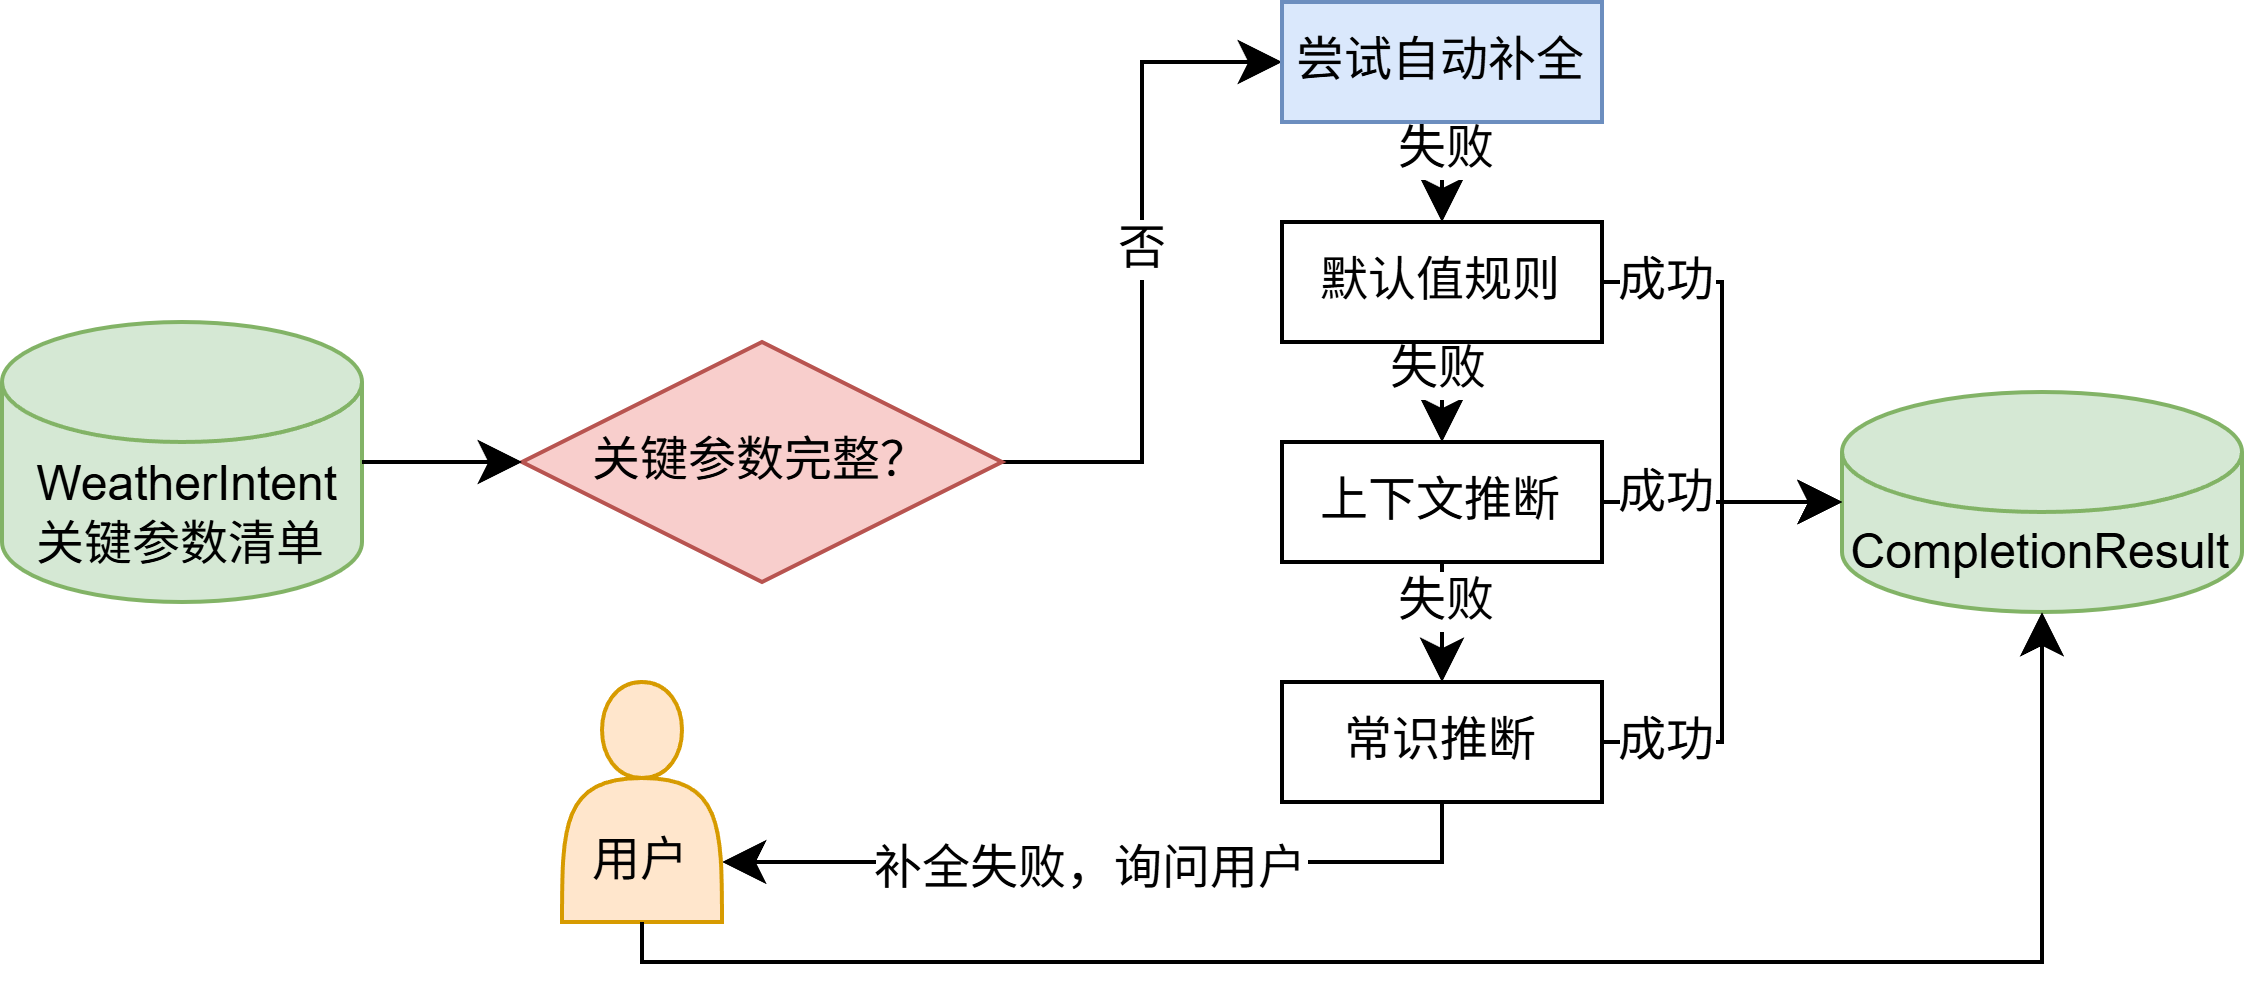
\includegraphics[width=0.78\linewidth]{figures/三档补全策略流程图}
    \caption{三档补全策略流程示意图}
    \label{fig:completion-three-tier}
\end{figure}

\subsubsection*{3.3.4 \quad 容错回退与可观测性}

\texttt{complete\_\bk{}intent} 函数同样实现了与 \texttt{recognize\_\bk{}intent}
对称的容错回退。当结构化输出多次返回 \texttt{None} 或抛出异常时，
函数返回 \texttt{is\_\bk{}complete=\bk{}True} 加原意图原样透传的兜底结果，
让 ReAct 循环可以继续推进，避免在意图理解前置就因偶发故障而
中止整个对话。这一兜底策略的代价是该次查询将放弃参数补全的
可解释性，但保证了系统级可用性。

可观测性是分层架构的另一项工程价值。每次 \texttt{recognize\_\bk{}intent}
与 \texttt{complete\_\bk{}intent} 的输入输出在 \texttt{run\_\bk{}agent} 函数
中以独立段落打印到日志，便于评测与生产排障时定位失败究竟发生在
哪一阶段。LangChain 框架 \cite{ref15} 提供的 \texttt{create\_\bk{}agent}
接口允许 ReAct 循环本身的中间状态以 stream 模式实时输出，与
意图识别加补全两阶段日志合并形成 4 阶段可追溯链条：原始查询、
\texttt{WeatherIntent}、\texttt{CompletionResult}、ReAct 工具
调用与最终回答。这一链条在
\ref{sec:e2e-eval} 节端到端评测中被进一步利用，作为
\texttt{e2e\_\bk{}intent\_\bk{}cache} 与 \texttt{e2e\_\bk{}agent\_\bk{}cache} 两层
缓存的天然切分点。

